\begin{figure*}[tb]
  \centering
  \subfloat[\label{nonrandom}Ordered Dispatch]{
    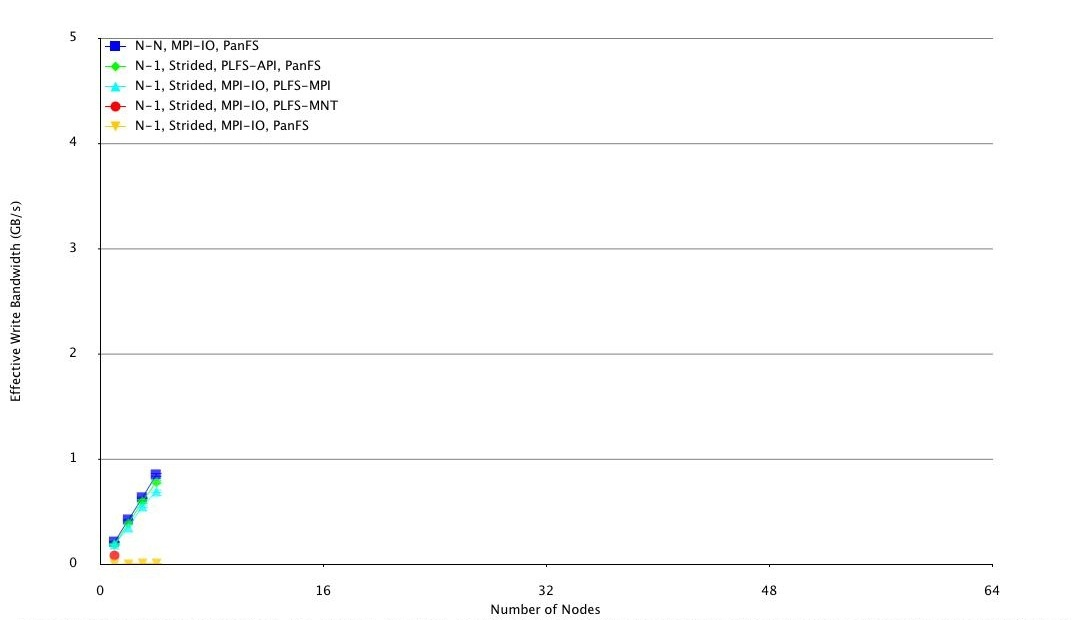
\includegraphics[width=0.3\textwidth,height=\figheight]{dbvizGraphsAndConfigs/pointsLTE4.jpg}
  }
  \subfloat[\label{random}Random Dispatch]{
    \includegraphics[width=0.3\textwidth,height=\figheight]{dbvizGraphsAndConfigs/random4Pts.jpg}
  }
  \subfloat[\label{random-full}Final Results]{
    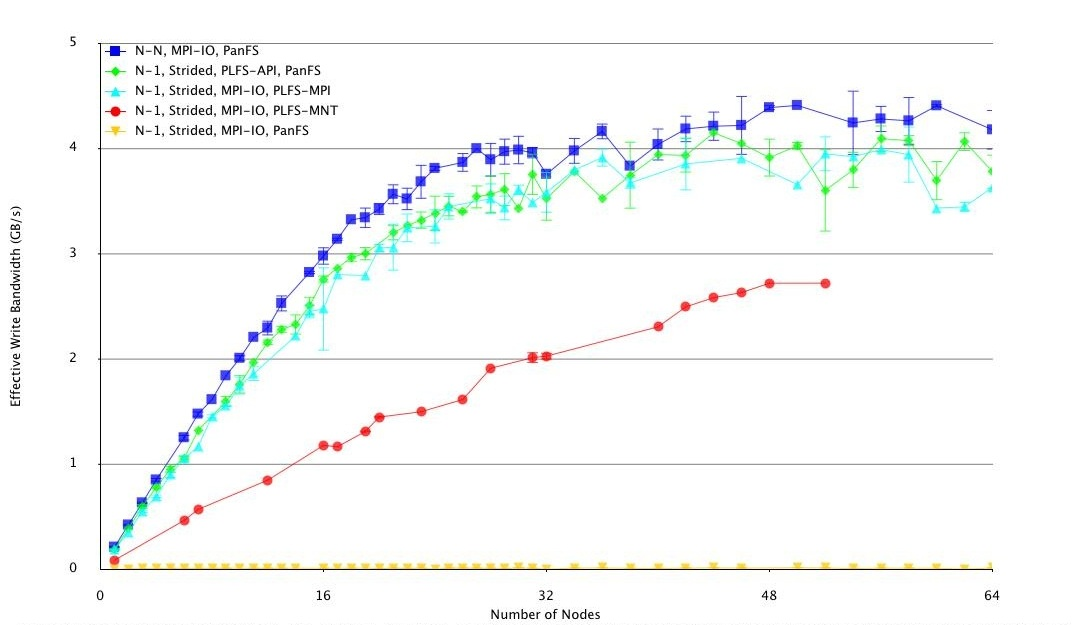
\includegraphics[width=0.3\textwidth,height=\figheight]{dbvizGraphsAndConfigs/allPoints.jpg}
  }
  \mycaption{fig-random}{Harnessing Randomness.}{
These three graphs illustrate the value of randomizing the generated commands
before dispatching them.  The graphs on the left and the middle were created
after only sixteen \subs\ were completed; the left-most is the graph produced when
the commands are dispatched in the order of their generation whereas the middle
graph was produced when the commands were randomly dispatched.  Finally, the
graph on the right shows the final results after all 492 \subs\ were completed.
By providing a much better approximation of the final graph, randomized 
commands allow computational steering much earlier in the experiment lifecycle.
}
\end{figure*}

